\chapter{Resultados experimentales}

En este capítulo se presentan los resultados obtenidos durante la evaluación de los modelos MobileNetV3 Small y EfficientNetV2B0.
El análisis considera tanto el desempeño de clasificación como el comportamiento de los modelos al ejecutarse directamente en los
dispositivos móviles definidos en la metodología. De esta manera, los resultados permiten observar no solo la calidad de las
predicciones, sino también la viabilidad práctica de cada arquitectura dentro de una aplicación Android.

\section{Resultados del entrenamiento de los modelos}

En esta sección se presentan los resultados obtenidos durante el entrenamiento de los modelos seleccionados para la aplicación móvil.
Estos resultados permiten observar el comportamiento de cada arquitectura sobre el conjunto de datos PlantVillage antes de su
conversión e integración en la aplicación Android. De esta manera, el análisis no se limita únicamente a la ejecución en el dispositivo, sino que
también considera el desempeño alcanzado por los modelos durante la etapa de entrenamiento y evaluación sobre el conjunto de prueba.

El entrenamiento de ambos modelos se ejecutó en modo completo, es decir sobre el total del conjunto de datos. En los dos casos se conservó la división de 43.442 imágenes para
entrenamiento, 5.430 para validación y 5.431 para prueba, usando la semilla 123 para mantener una comparación directa entre las
arquitecturas.

\subsection{Modelo MobileNetV3 Small}

Como se espeficio en la metodologia la variante seleccionada de la familia MobileNetV3 fue MobileNetV3 Small. Para este modelo se utilizaron imágenes de
entrada de 224x224 píxeles, pesos iniciales preentrenados en ImageNet y un preprocesamiento en el rango [-1, 1], el mismo que fue
utilizado posteriormente en la aplicación Android.

\subsubsection{Configuración del entrenamiento}

La tabla \ref{tab:mobilenet_training_results} resume los principales resultados del entrenamiento y exportación del modelo
MobileNetV3 Small. A diferencia de EfficientNetV2B0, este modelo conserva un tamaño final menor, lo que resulta importante para su
uso dentro de una aplicación móvil.

\begin{table}[H]
    \centering
    \caption{Resumen de entrenamiento y exportación del modelo MobileNetV3 Small.}
    \label{tab:mobilenet_training_results}
    \begin{tabular}{>{\raggedright\arraybackslash}p{6cm} >{\centering\arraybackslash}p{6cm}}
        \hline
        \textbf{Atributo} & \textbf{Resultado} \\
        \hline
        Arquitectura & MobileNetV3 Small \\
        Tamaño de entrada & 224x224 píxeles \\
        Número de clases & 38 \\
        División del conjunto de datos & 80\% entrenamiento, 10\% validación, 10\% prueba \\
        Imágenes de entrenamiento & 43442 \\
        Imágenes de validación & 5430 \\
        Imágenes de prueba & 5431 \\
        Preprocesamiento & Normalización en el rango [-1, 1] \\
        Épocas de entrenamiento de cabeza & 10 \\
        Épocas de ajuste fino & 10 \\
        Capas descongeladas en ajuste fino & Últimas 30 capas del backbone \\
        Mejor exactitud de validación & 0,9831 \\
        Exactitud en prueba & 0,9856 \\
        Pérdida en prueba & 0,0485 \\
        Tamaño del modelo TFLite FP32 & 3,67 MB \\
        Tamaño del modelo TFLite FP16 & 1,91 MB \\
        \hline
    \end{tabular}
\end{table}

\subsubsection{Evolución del entrenamiento}

El entrenamiento también se desarrolló en dos fases. En la primera fase se congeló el backbone preentrenado y se entrenó la cabeza
de clasificación, permitiendo que el modelo adaptara la salida final a las 38 clases de PlantVillage. En la segunda fase se realizó
el ajuste fino, descongelando las últimas 30 capas del backbone con una tasa de aprendizaje menor. Las capas de normalización por
lotes se mantuvieron congeladas durante esta etapa, con el fin de conservar la estabilidad del modelo y evitar cambios bruscos en las
estadísticas aprendidas durante el preentrenamiento.

La figura \ref{fig:mobilenet_training_graph} muestra las curvas de exactitud y pérdida del entrenamiento. En la curva de exactitud se
observa un crecimiento rápido durante las primeras épocas, pasando de valores cercanos a 0,84 en entrenamiento a valores superiores a
0,96 después de pocas iteraciones. Luego, durante el ajuste fino, la mejora se vuelve más gradual hasta alcanzar una exactitud de
validación de 0,9831. En la curva de pérdida se observa una disminución continua tanto en entrenamiento como en validación, sin
una separación marcada entre ambas curvas. Este comportamiento muestra una convergencia estable y no evidencia un sobreajuste fuerte
durante la ejecución registrada.

\begin{figure}[H]
    \centering
    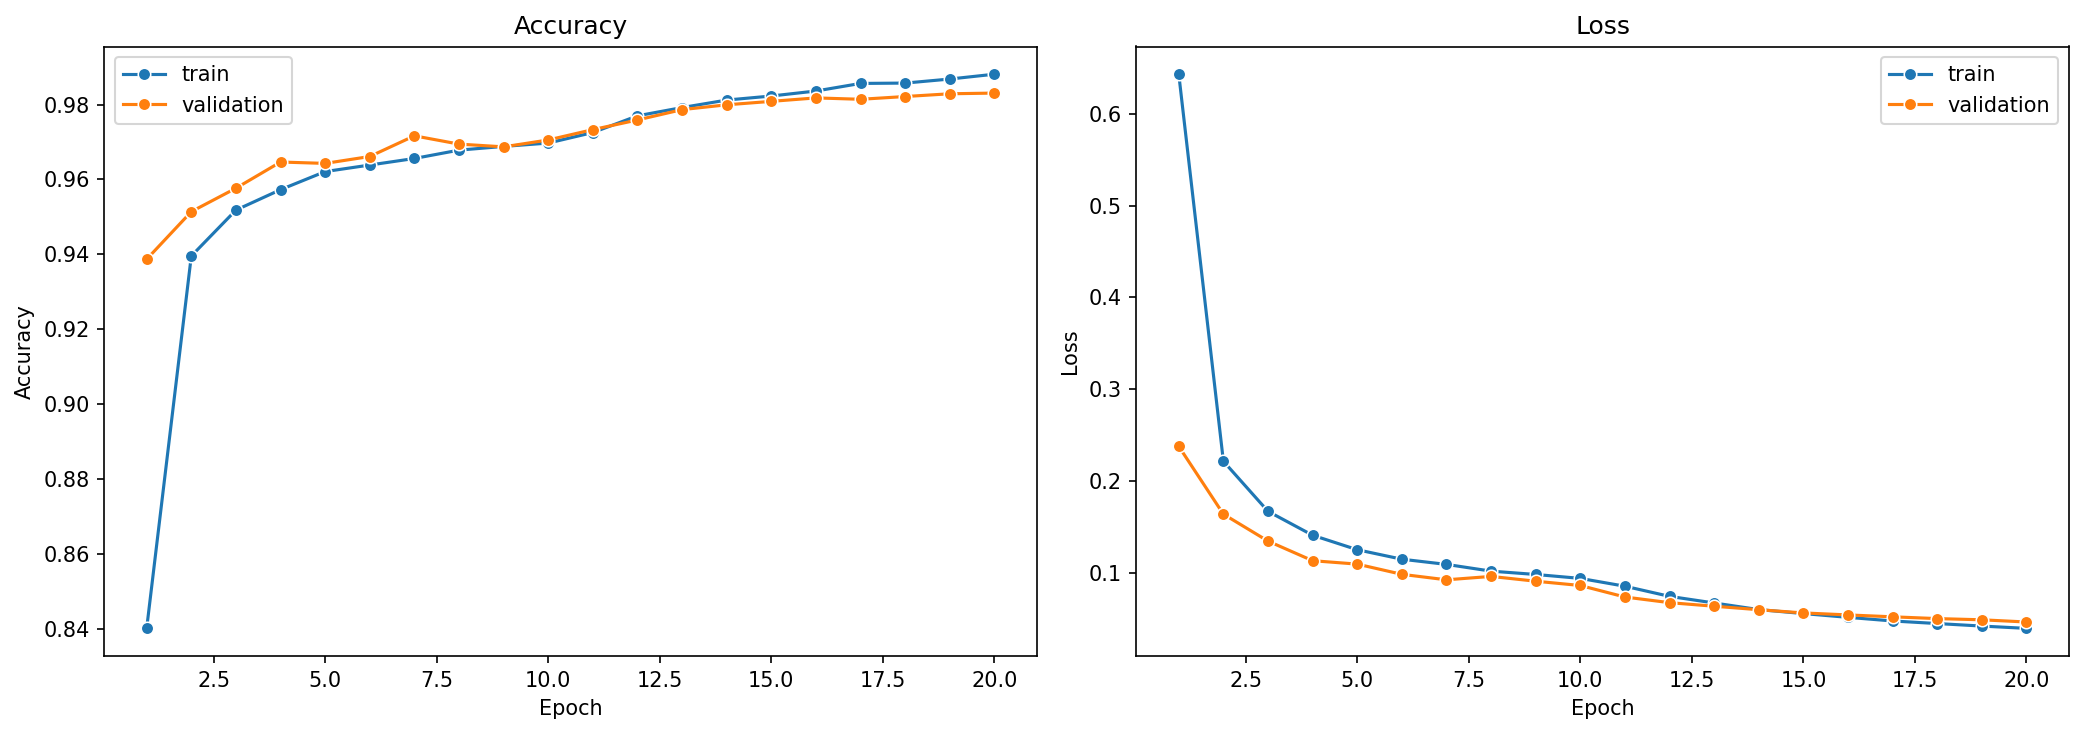
\includegraphics[width=1\textwidth]{../MobileNet/training graph.png}
    \caption{Curvas de exactitud y pérdida durante el entrenamiento de MobileNetV3 Small.\label{fig:mobilenet_training_graph}}
\end{figure}

\subsubsection{Evaluación en el conjunto de prueba}

Al evaluar el modelo sobre el conjunto de prueba, MobileNetV3 Small alcanzó una exactitud de 0,9856 y una pérdida de 0,0485. Este
resultado muestra que el modelo logró generalizar adecuadamente sobre imágenes que no fueron utilizadas durante el entrenamiento. Al
relacionar este valor con las curvas de exactitud y pérdida, se observa que el comportamiento del modelo fue consistente entre
entrenamiento, validación y prueba, ya que la pérdida se mantuvo baja y la exactitud de validación alcanzó valores cercanos a los
obtenidos en el conjunto de prueba.

La matriz de confusión obtenida para MobileNetV3 Small se presenta en la figura \ref{fig:mobilenet_confusion_matrix}. En términos
generales, la diagonal principal concentra la mayor parte de las predicciones correctas, lo que coincide con la exactitud global
obtenida. Las confusiones restantes se concentran principalmente en clases visualmente cercanas, especialmente en enfermedades de
tomate y maíz, donde las hojas pueden presentar manchas, cambios de coloración o lesiones con patrones similares.

\begin{figure}[H]
    \centering
    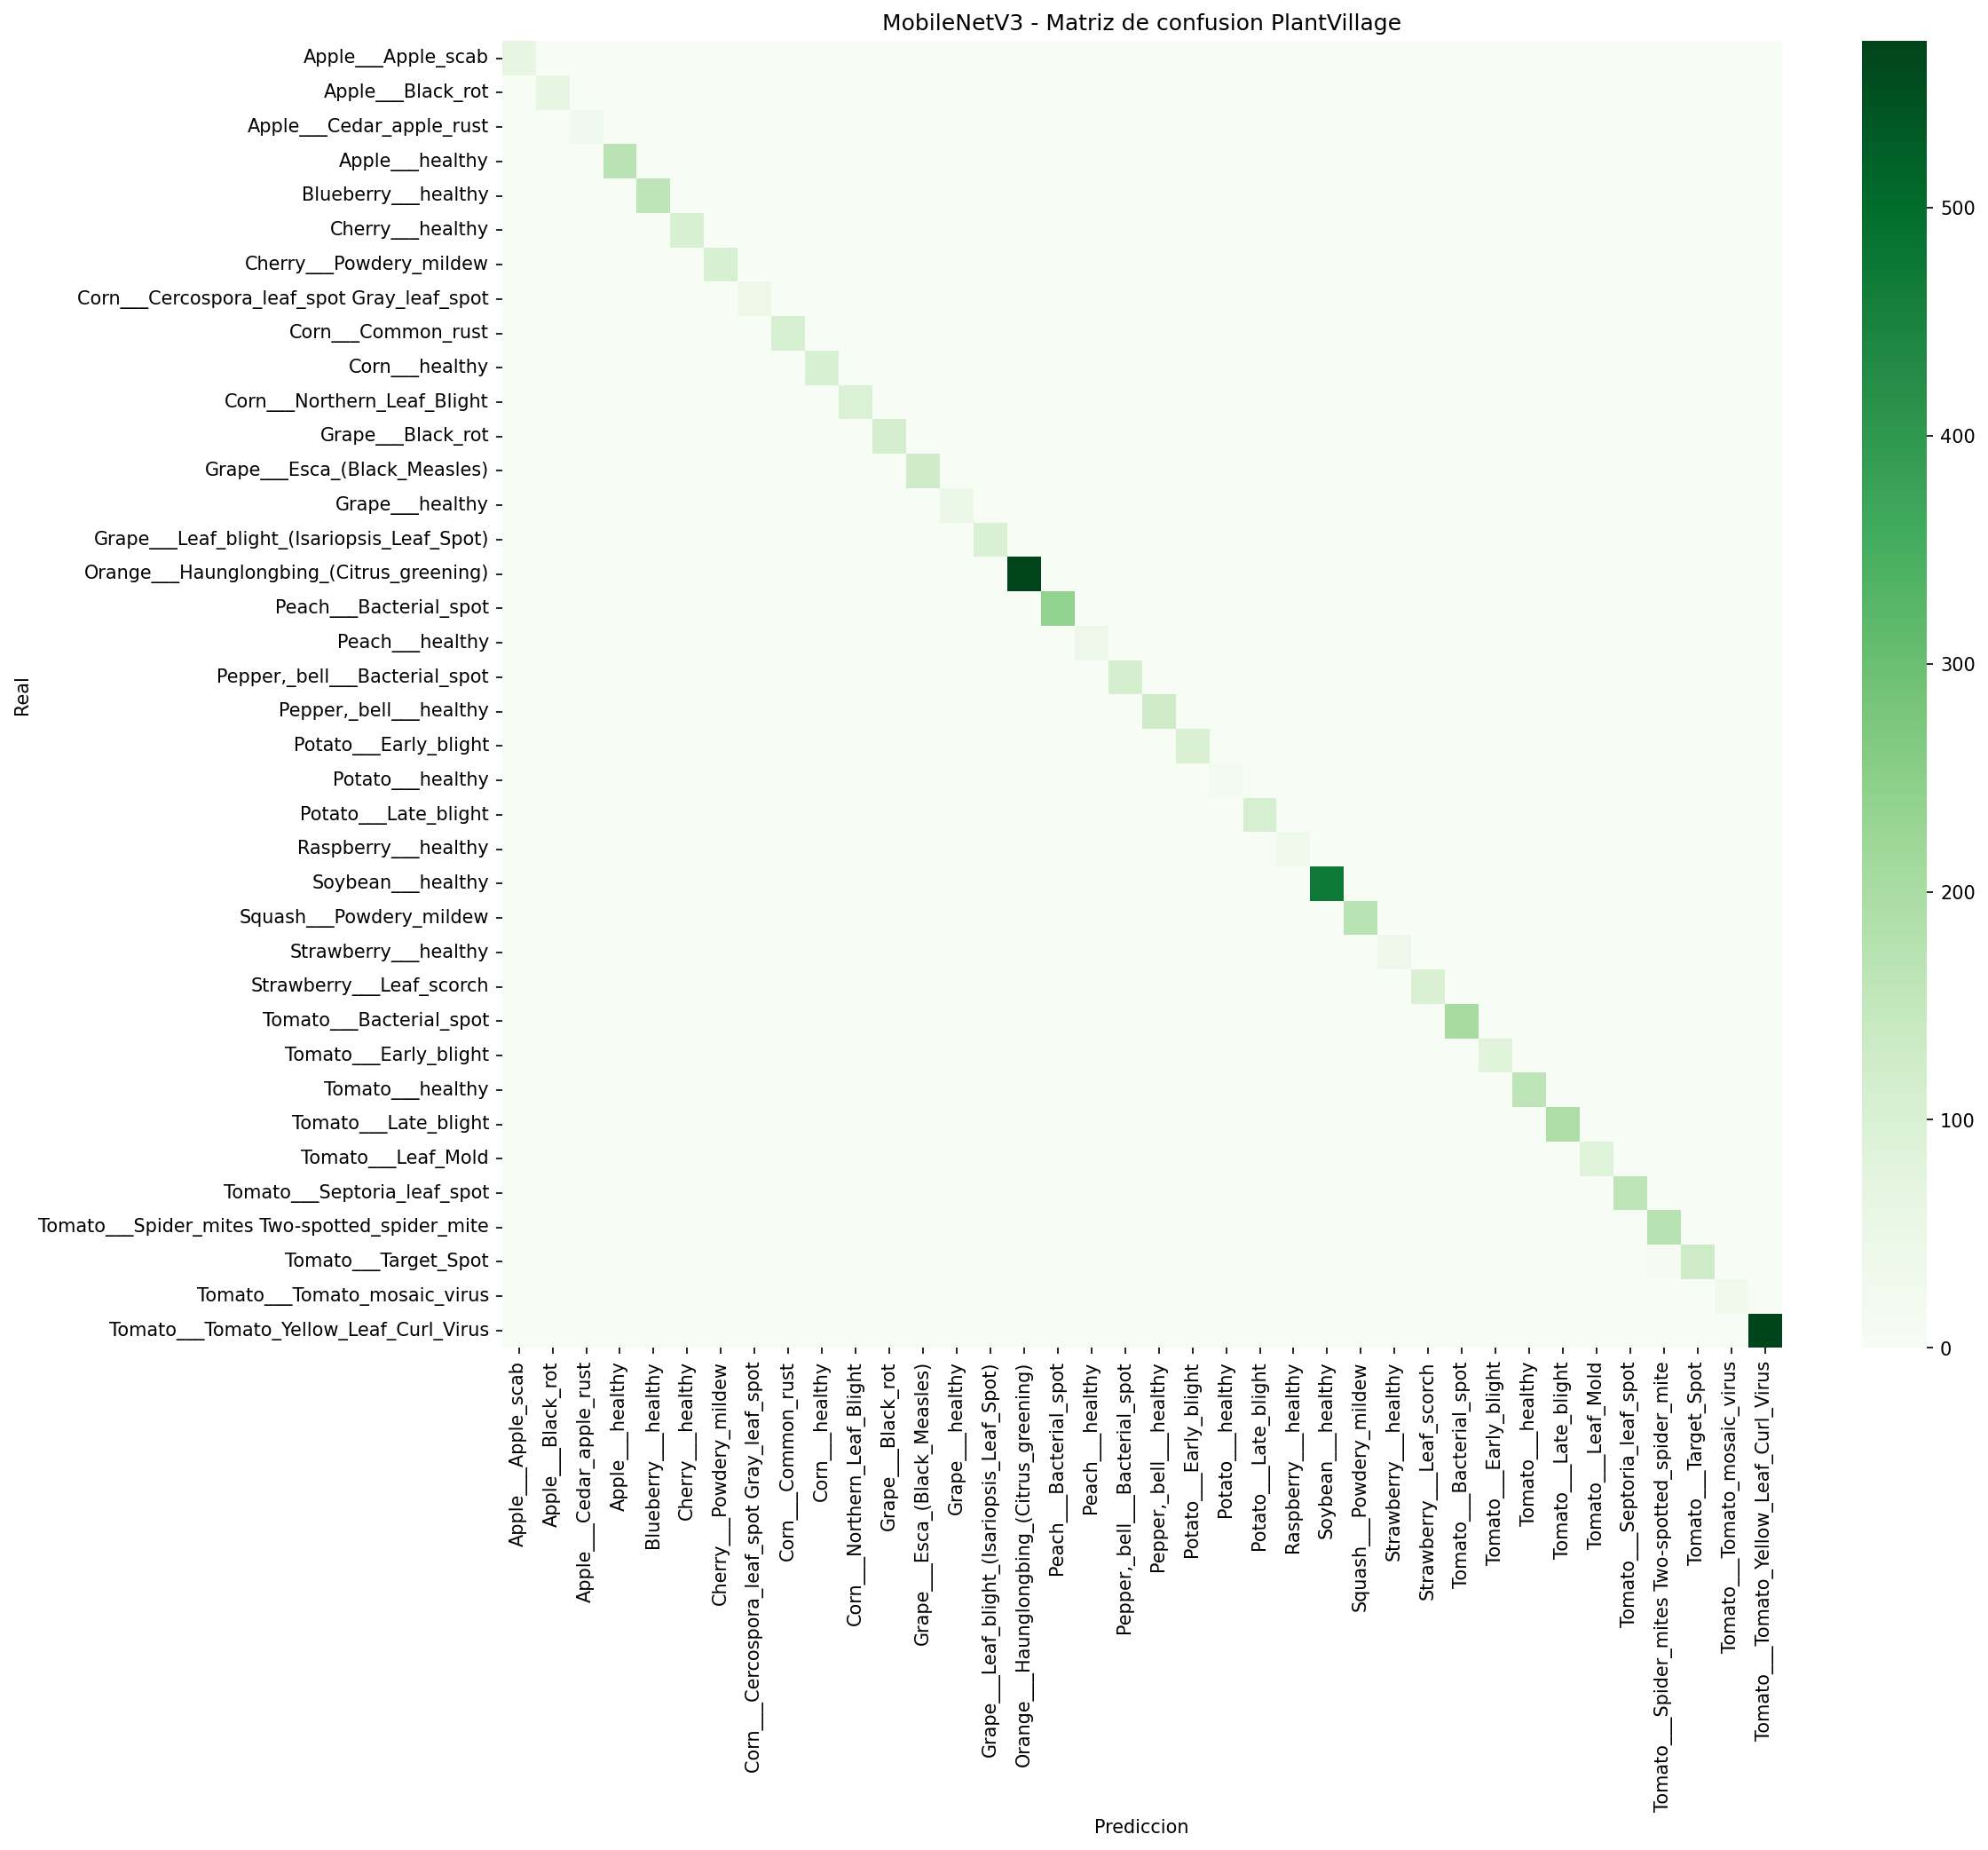
\includegraphics[width=0.95\textwidth]{../MobileNet/confussion_matrix.png}
    \caption{Matriz de confusión del modelo MobileNetV3 Small sobre el conjunto de prueba de PlantVillage.\label{fig:mobilenet_confusion_matrix}}
\end{figure}

\subsubsection{Exportación del modelo}

Después del entrenamiento, el modelo fue exportado a TensorFlow Lite en formato FP32 y FP16. La versión FP16 redujo el tamaño del
archivo de 3,67 MB a 1,91 MB, lo que representa una ventaja importante frente a EfficientNetV2B0 para el despliegue móvil. Esta
diferencia permite que MobileNetV3 Small sea más liviano dentro de la aplicación y mantenga un desempeño de clasificación alto sin
incrementar de forma significativa el tamaño del modelo integrado.

\subsection{Modelo EfficientNetV2B0}

EfficientNetV2B0 fue entrenado como arquitectura de comparación frente a MobileNetV3 Small, manteniendo el mismo conjunto de clases,
la misma división de los datos y el mismo criterio de evaluación descrito en la metodología. Para este modelo se utilizó la variante
B0, con imágenes de entrada de 224x224 píxeles y pesos iniciales preentrenados en ImageNet. A diferencia de MobileNetV3 Small, el
preprocesamiento de EfficientNetV2B0 se realizó normalizando los valores de los píxeles en el rango [0, 1], por lo que esta
diferencia también se conservó durante la integración del modelo en la aplicación móvil.

\subsubsection{Configuración del entrenamiento}

La tabla \ref{tab:efficientnet_training_results} resume los principales resultados del entrenamiento y exportación del modelo
EfficientNetV2B0, considerando tanto la configuración utilizada como las métricas obtenidas sobre el conjunto de prueba.

\begin{table}[H]
    \centering
    \caption{Resumen de entrenamiento y exportación del modelo EfficientNetV2B0.}
    \label{tab:efficientnet_training_results}
    \begin{tabular}{>{\raggedright\arraybackslash}p{6cm} >{\centering\arraybackslash}p{6cm}}
        \hline
        \textbf{Atributo} & \textbf{Resultado} \\
        \hline
        Arquitectura & EfficientNetV2B0 \\
        Variante & B0 \\
        Tamaño de entrada & 224x224 píxeles \\
        Número de clases & 38 \\
        División del conjunto de datos & 80\% entrenamiento, 10\% validación, 10\% prueba \\
        Imágenes de entrenamiento & 43442 \\
        Imágenes de validación & 5430 \\
        Imágenes de prueba & 5431 \\
        Preprocesamiento & Normalización en el rango [0, 1] \\
        Épocas de entrenamiento de cabeza & 15 \\
        Épocas de ajuste fino & 10 \\
        Capas descongeladas en ajuste fino & Últimas 20 capas del backbone \\
        Mejor exactitud de validación & 0,9851 \\
        Exactitud en prueba & 0,9847 \\
        Pérdida en prueba & 0,0490 \\
        Precisión macro & 0,9823 \\
        Recall macro & 0,9758 \\
        F1-score macro & 0,9784 \\
        Errores en prueba & 83 de 5431 imágenes \\
        Tamaño del modelo TFLite FP32 & 22,52 MB \\
        Tamaño del modelo TFLite FP16 & 11,33 MB \\
        \hline
    \end{tabular}
\end{table}

La arquitectura final tuvo 5.973.110 parámetros, de los cuales
en la primera fase solo se entrenaron 51.238 correspondientes a la cabeza de clasificación.


\subsubsection{Evolución del entrenamiento}

El entrenamiento se organizó en dos fases. En la primera fase se congeló el backbone preentrenado y se entrenó únicamente la cabeza
de clasificación agregada para las 38 clases de PlantVillage. Esta etapa inició con una exactitud de validación de 0,9586 en la
primera época y finalizó con 0,9805 en la época 15. Durante esta fase se observaron pequeñas mesetas en la mejora de la validación,
por lo que el ajuste automático de la tasa de aprendizaje redujo el valor inicial de 1e-3 a 3e-4 y posteriormente a 9e-5. Después de
estas reducciones, el modelo volvió a mejorar, lo que muestra que el mecanismo de reducción de learning rate ayudó a continuar la
convergencia.

Posteriormente, en la fase de ajuste fino, se descongelaron las últimas capas del backbone con una tasa de aprendizaje de 1e-5,
manteniendo congeladas las capas de normalización por lotes para evitar cambios bruscos en las estadísticas aprendidas durante el
preentrenamiento. Esta segunda fase aumentó la exactitud de validación desde 0,9805 hasta 0,9851, obtenida en la época 24. La época
25 presentó una disminución leve en la exactitud de validación, mientras que la exactitud de entrenamiento continuó aumentando, por
lo que el mejor checkpoint correspondió a la época 24.

La figura \ref{fig:efficientnet_training_graph} muestra las curvas de exactitud y pérdida durante las dos fases del entrenamiento.
En la curva de exactitud se observa una mejora rápida durante las primeras épocas, seguida de un crecimiento más gradual. En la curva
de pérdida, tanto el error de entrenamiento como el de validación disminuyen de forma estable, sin una separación marcada entre ambas
curvas. Este comportamiento indica que el modelo logró adaptarse al conjunto PlantVillage sin evidenciar un sobreajuste fuerte durante
la ejecución registrada.

\begin{figure}[H]
    \centering
    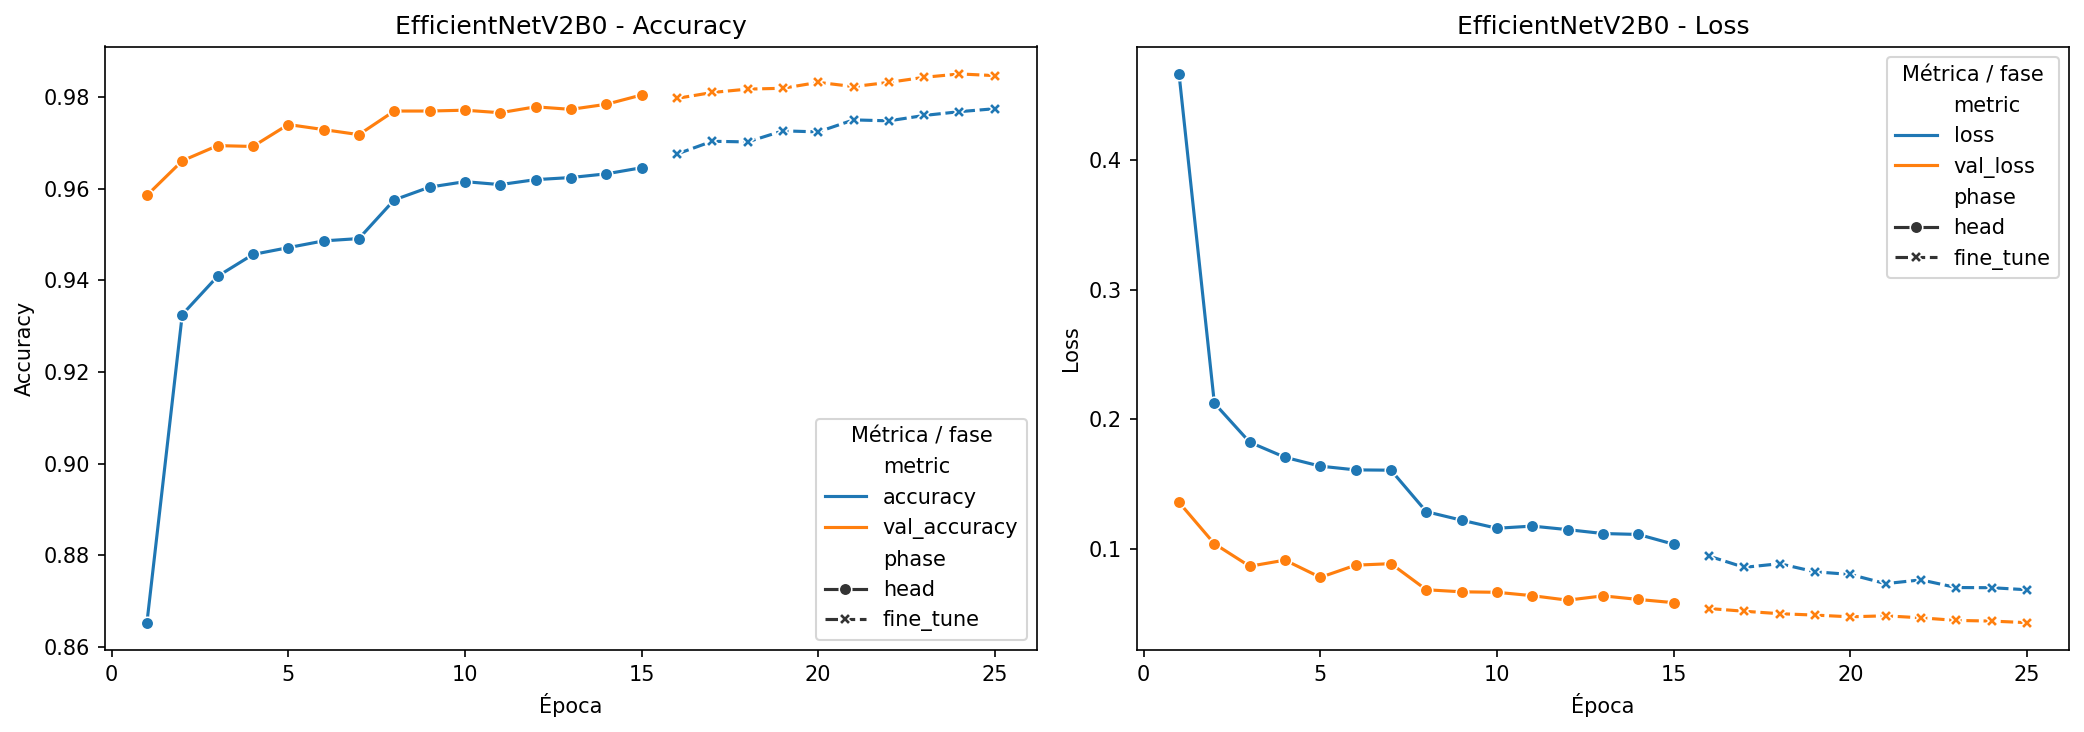
\includegraphics[width=1\textwidth]{../EfficientNet/training_graph_v2b0.png}
    \caption{Curvas de exactitud y pérdida durante el entrenamiento de EfficientNetV2B0.\label{fig:efficientnet_training_graph}}
\end{figure}

\subsubsection{Evaluación en el conjunto de prueba}

Al evaluar el mejor checkpoint sobre el conjunto de prueba, el modelo alcanzó una exactitud de 0,9847 y una pérdida de 0,0490. En
términos generales, este resultado muestra que EfficientNetV2B0 consiguió un desempeño alto sobre PlantVillage, con 83 errores en
5.431 imágenes evaluadas. Además, las métricas agregadas se mantuvieron cercanas entre sí, con una precisión macro de 0,9823, recall
macro de 0,9758 y F1-score macro de 0,9784.

Aunque el resultado global fue alto, el análisis por clase muestra que los errores no se distribuyeron de manera uniforme. La tabla
\ref{tab:efficientnet_weak_classes} presenta las clases con F1-score menor a 0,96, que corresponden a los casos donde el modelo tuvo
mayor dificultad relativa.

\begin{table}[H]
    \centering
    \caption{Clases con menor desempeño relativo en EfficientNetV2B0.}
    \label{tab:efficientnet_weak_classes}
    \begin{tabular}{>{\raggedright\arraybackslash}p{5.7cm}
                    >{\centering\arraybackslash}p{1.6cm}
                    >{\centering\arraybackslash}p{1.6cm}
                    >{\centering\arraybackslash}p{1.6cm}
                    >{\centering\arraybackslash}p{1.6cm}}
        \hline
        \textbf{Clase} & \textbf{Prec.} & \textbf{Recall} & \textbf{F1} & \textbf{Soporte} \\
        \hline
        Potato healthy & 1,0000 & 0,7273 & 0,8421 & 11 \\
        Tomato Target Spot & 0,8855 & 0,8855 & 0,8855 & 131 \\
        Corn Cercospora leaf spot Gray leaf spot & 0,9375 & 0,9000 & 0,9184 & 50 \\
        Tomato Early blight & 0,9691 & 0,8952 & 0,9307 & 105 \\
        Tomato Septoria leaf spot & 0,9459 & 0,9396 & 0,9428 & 149 \\
        Tomato Leaf Mold & 0,9341 & 0,9551 & 0,9444 & 89 \\
        Tomato Spider mites Two-spotted spider mite & 0,9382 & 0,9543 & 0,9462 & 175 \\
        \hline
    \end{tabular}
\end{table}

En la tabla, Prec. corresponde a precisión.

El caso de Potato healthy (Papa sana) fue el de menor F1-score; sin embargo, esta clase tuvo solo 11 ejemplos en el conjunto de prueba, por lo
que cada error individual tuvo un impacto alto sobre el recall. En cambio, Tomato Target Spot representa un caso más relevante para
el análisis, debido a que tuvo un soporte mayor y presentó confusiones con otras enfermedades de tomate. Este patrón también se
observó en Tomato Septoria leaf spot, Tomato Leaf Mold y Tomato Spider mites, donde las lesiones foliares pueden tener una apariencia
visual similar. En maíz, la confusión principal apareció entre Corn Cercospora leaf spot Gray leaf spot y Corn Northern Leaf Blight,
lo cual es consistente con la similitud visual entre lesiones alargadas y manchas grises en las hojas.

La matriz de confusión obtenida para EfficientNetV2B0 se presenta en la figura \ref{fig:efficientnet_confusion_matrix}. Esta matriz
permite identificar visualmente las clases en las que el modelo concentró la mayor parte de sus aciertos y los casos en los que se
presentaron confusiones entre enfermedades o cultivos con características visuales similares. Este análisis es relevante porque una
exactitud global alta no siempre evidencia los errores específicos que pueden aparecer en clases particulares.

\begin{figure}[H]
    \centering
    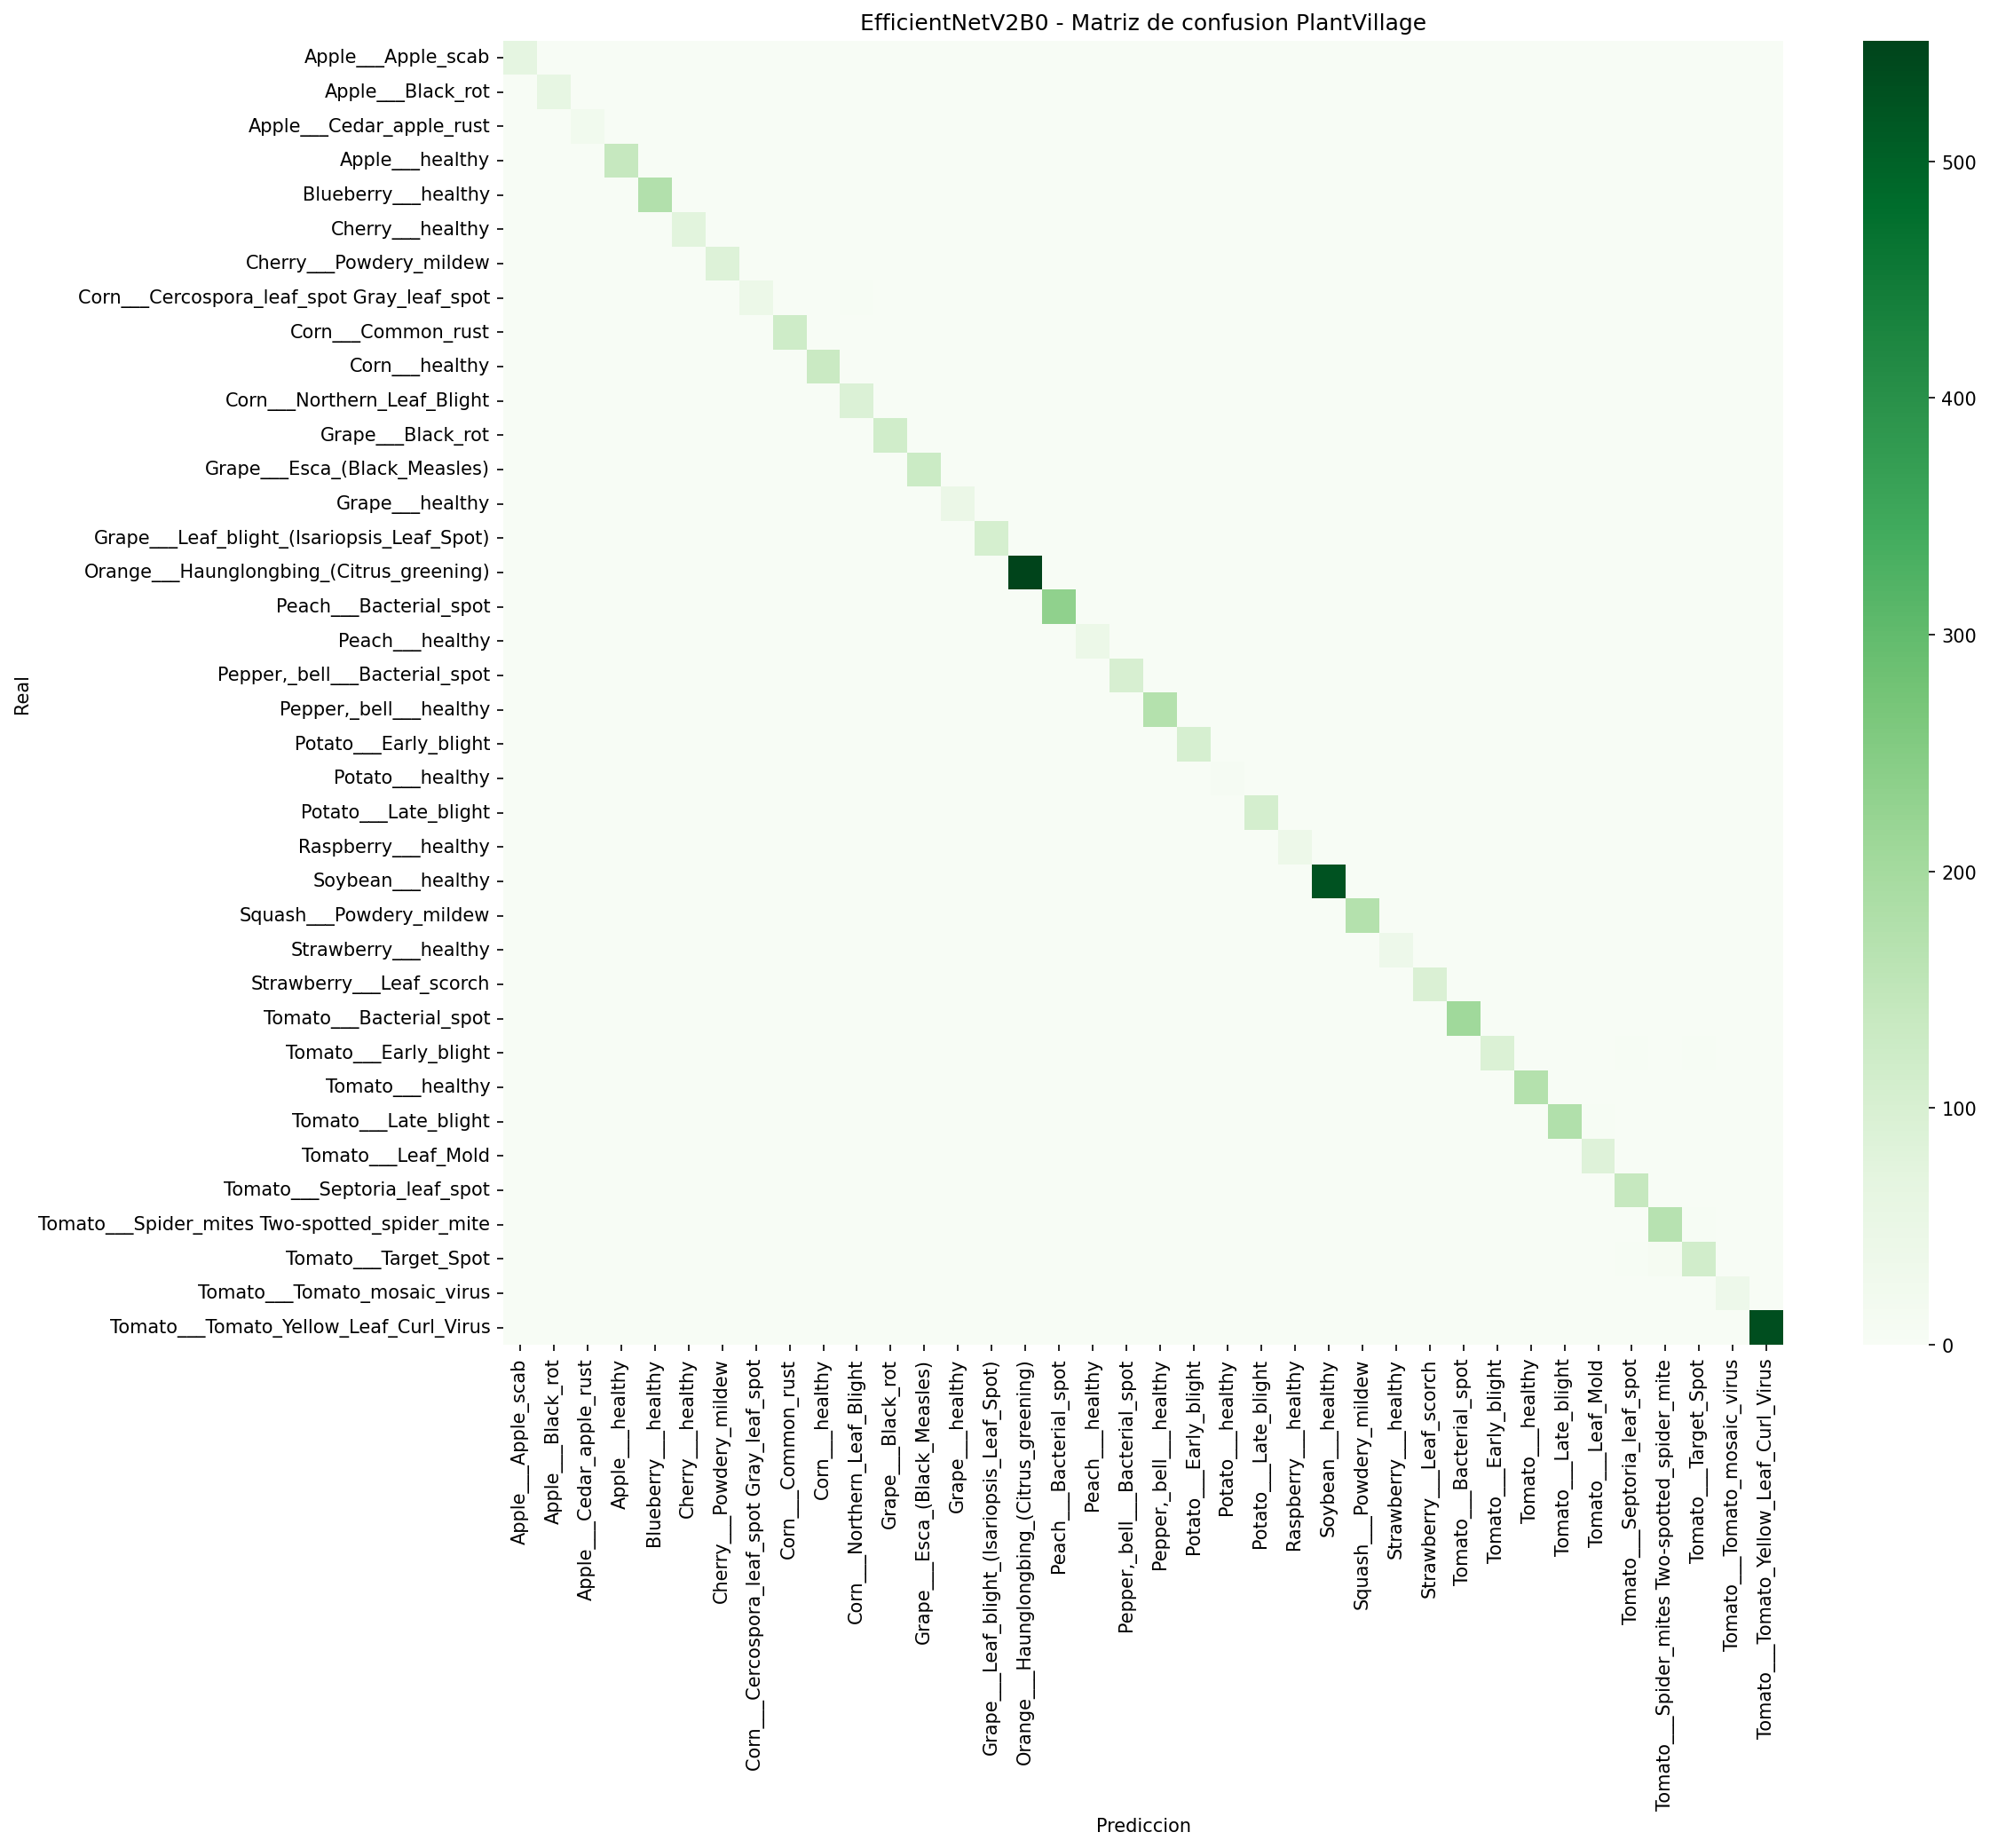
\includegraphics[width=0.95\textwidth]{../EfficientNet/confusion_matrix_v2b0.png}
    \caption{Matriz de confusión del modelo EfficientNetV2B0 sobre el conjunto de prueba de PlantVillage.\label{fig:efficientnet_confusion_matrix}}
\end{figure}

\subsubsection{Exportación del modelo}

Después del entrenamiento, el modelo fue exportado a TensorFlow Lite en formato FP32 y FP16. La versión FP16 redujo el tamaño del
archivo aproximadamente a la mitad, pasando de 22,52 MB a 11,33 MB. Esta reducción es importante para el despliegue en dispositivos
móviles, ya que disminuye el espacio requerido por el modelo dentro de la aplicación y facilita su distribución sin modificar la
estructura general de la arquitectura entrenada. Sin embargo, este modelo requiere conservar el preprocesamiento en el rango [0, 1],
por lo que su uso en Android depende de aplicar una normalización diferente a la utilizada por MobileNetV3 Small.

\section{Aplicación móvil}
En la figura \ref{fig:app_screenshots} se muestran capturas de pantalla de la aplicación móvil desarrollada para la ejecución de
inferencias en los dispositivos. La pantalla inicial (captura a) permite seleccionar el modelo que se desea probar, ya sea
MobileNetV3 Small o EfficientNetV2B0. Desde esta misma vista, el usuario puede ingresar la imagen al modelo mediante dos opciones:
cargar una fotografía desde la galería del dispositivo (captura b) o capturar una imagen directamente desde la cámara de la
aplicación (captura c). En la pantalla de captura se mantiene un área de enfoque que orienta al usuario para ubicar la hoja dentro
de la región de análisis, con el fin de facilitar una entrada más adecuada para el proceso de inferencia.

\begin{figure}[H]
    \centering
    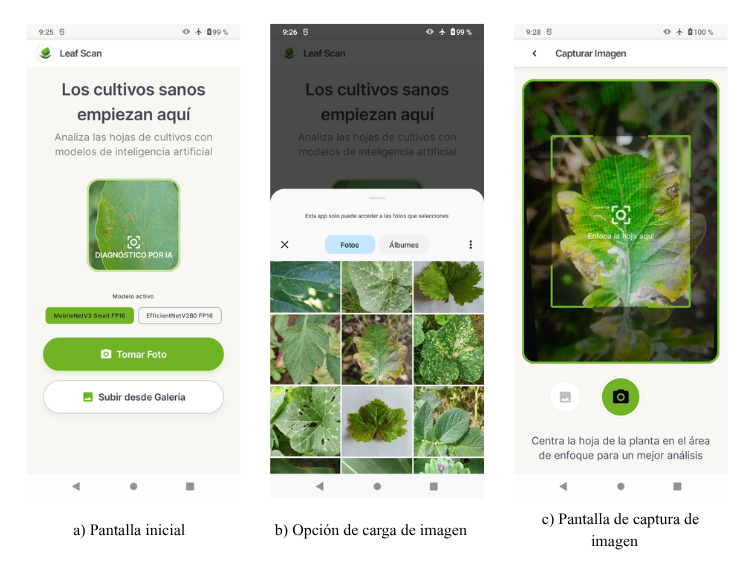
\includegraphics[width=1\textwidth]{images/app_screenshots.png}
    \caption{Pantallas iniciales de la aplicación móvil: selección del modelo, carga desde galería y captura de imagen.\label{fig:app_screenshots}}
\end{figure}


Posteriormente, en la figura \ref{fig:app_screenshots_2} se presenta el flujo de análisis de la imagen. La pantalla de análisis
(captura a) muestra la imagen seleccionada y el avance de la ejecución del modelo, de manera que el usuario pueda identificar que la
inferencia se encuentra en proceso. Cuando la predicción obtiene una confianza igual o superior al umbral definido del 50\%, se
presenta la pantalla de resultado (captura b), en la cual se indica la clase asignada, el porcentaje de confianza asociado y una
descripción breve relacionada con el diagnóstico obtenido.

En caso de que la confianza de la predicción sea menor al 50\%, o si durante la ejecución del modelo se presenta un error, la
aplicación muestra un mensaje de error en la pantalla de análisis (captura c). Aquí se informa que no fue posible clasificar la 
imagen y se habilita la
opción de reintento, permitiendo al usuario tomar o seleccionar una nueva fotografía. De esta forma, la interfaz mantiene un flujo
simple para la prueba de los modelos, desde la selección de la imagen hasta la visualización del diagnóstico o la repetición del
proceso cuando la entrada no permite una inferencia confiable.

\begin{figure}[H]
    \centering
    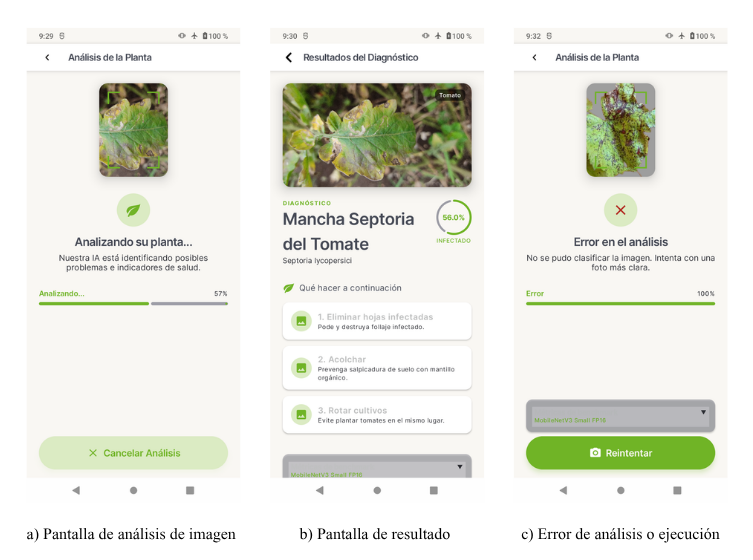
\includegraphics[width=1\textwidth]{images/app_screenshots_2.png}
    \caption{Pantallas de análisis, resultado y error durante la inferencia en la aplicación móvil.\label{fig:app_screenshots_2}}
\end{figure}

\section{Resultados de ejecución en dispositivo}

    La tabla \ref{tab:motog_execution_results} presenta las mediciones obtenidas en el dispositivo Moto G30 durante tres sesiones de
    evaluación. En cada sesión se ejecutaron ambos modelos bajo el mismo protocolo de prueba, registrando variables asociadas al estado del
dispositivo y al tiempo de inferencia. Durante la ejecucion del protocolo de prueba, se mantuvo el dispositivo en un entorno controlado, 
evitando la ejecución de otras aplicaciones que pudieran afectar el rendimiento. Durante la 
ejecucion de las tres sesiones se mantuvo el mismo nivel de brillo establecido en 60\% y se deshabilitaron las conexiones inalámbricas para evitar interferencias externas,
tambien se desctivo el modo Rendimiento permitiendo el uso de todos los núcleos del procesador.
En ninguna de las sesiones se registraron crashes de la aplicación, ni por errores de codigo ni por falta de recursos.
En las tablas, MNetV3 corresponde a MobileNetV3 Small y EffNet corresponde a EfficientNetV2B0.

\begin{table}[H]
    \centering
    \caption{Resultados de ejecución de MobileNetV3 Small y EfficientNetV2B0 en Moto G30.}
    \label{tab:motog_execution_results}
    \scriptsize
    \resizebox{\textwidth}{!}{%
    \begin{tabular}{>{\raggedright\arraybackslash}p{3.2cm}
                    >{\centering\arraybackslash}p{1.8cm}
                    >{\centering\arraybackslash}p{1.8cm}
                    >{\centering\arraybackslash}p{1.8cm}
                    >{\centering\arraybackslash}p{1.8cm}
                    >{\centering\arraybackslash}p{1.8cm}
                    >{\centering\arraybackslash}p{1.8cm}}
        \hline
        \multicolumn{7}{c}{\textbf{Moto G30}} \\
        \hline
        \textbf{Métrica} & \multicolumn{2}{c}{\textbf{Sesión 1}} & \multicolumn{2}{c}{\textbf{Sesión 2}} & \multicolumn{2}{c}{\textbf{Sesión 3}} \\
        \hline
        & \textbf{MNetV3} & \textbf{EffNet} & \textbf{MNetV3} & \textbf{EffNet} & \textbf{MNetV3} & \textbf{EffNet} \\
        \hline
        Temperatura inicial (C) & 283 & 284 & 272 & 290 & 258 & 300 \\
        Temperatura final (C) & 296 & 316 & 295 & 324 & 295 & 313 \\
        Batería inicial (\%) & 100 & 79 & 72 & 65 & 50 & 65 \\
        Batería final (\%) & 77 & 68 & 63 & 55 & 37 & 51 \\
        Tiempo de inicialización (ms) & 3423 & 357 & 3220 & 319 & 3258 & 374 \\
        Warmup (ms) & 258,8 & 495,8 & 248 & 463,1 & 60,4 & 671,4 \\
        Latencia promedio (ms) & 24,8 & 273,6 & 31,9 & 276,8 & 35,3 & 272 \\
        Mediana P50 (ms) & 23,2 & 266,6 & 31 & 271,8 & 31,8 & 265,2 \\
        Percentil P95 (ms) & 36,9 & 311,4 & 52,5 & 323,9 & 69 & 318,1 \\
        Desviación estándar (ms) & 7,5 & 22,6 & 12,3 & 22,8 & 18,1 & 23,2 \\
        \hline
    \end{tabular}%
    }
\end{table}

La tabla \ref{tab:motog_cross_session_results} resume el promedio entre sesiones para las métricas principales de latencia en el
Moto G30. Aquí se observa de forma más directa la diferencia global entre ambos modelos, donde MobileNetV3 Small mantiene latencias promedio 
considerablemente menores, mientras que EfficientNetV2B0 presenta tiempos más altos y una variabilidad mayor. En términos de latencia promedio,
MobileNetV3 Small fue aproximadamente 8,94 veces más rápido que EfficientNetV2B0, lo que evidencia una brecha significativa en el rendimiento
de inferencia entre ambos modelos en este dispositivo móvil. Esta diferencia se mantiene también en la mediana P50 y el percentil P95, 
aunque con una variabilidad mayor en el caso de EfficientNetV2B0, lo que sugiere que este modelo no solo es más lento en promedio, sino que también
presenta una mayor inconsistencia en sus tiempos de inferencia.
\begin{table}[H]
    \centering
    \caption{Promedio entre sesiones de las métricas de ejecución en Moto G30.}
    \label{tab:motog_cross_session_results}
    \resizebox{\textwidth}{!}{%
    \begin{tabular}{>{\raggedright\arraybackslash}p{4cm}
                    >{\centering\arraybackslash}p{3cm}
                    >{\centering\arraybackslash}p{3cm}
                    >{\centering\arraybackslash}p{3cm}}
        \hline
        \textbf{Métrica} & \textbf{MNetV3} & \textbf{EffNet} & \textbf{Ratio Eff/MNV3} \\
        \hline
        Latencia promedio (ms) & 30,67 & 274,13 & 8,94x \\
        Mediana P50 (ms) & 28,67 & 267,87 & 9,34x \\
        Percentil P95 (ms) & 52,80 & 317,80 & 6,02x \\
        Desviación estándar (ms) & 12,63 & 22,87 & -- \\
        \hline
    \end{tabular}%
    }
\end{table}

La tabla \ref{tab:samsung_execution_results} presenta las mediciones obtenidas en el dispositivo Samsung Galaxy S23 durante las tres
sesiones de evaluación. 

\begin{table}[H]
    \centering
    \caption{Resultados de ejecución de MobileNetV3 Small y EfficientNetV2B0 en Samsung Galaxy S23.}
    \label{tab:samsung_execution_results}
    \scriptsize
    \resizebox{\textwidth}{!}{%
    \begin{tabular}{>{\raggedright\arraybackslash}p{3.2cm}
                    >{\centering\arraybackslash}p{1.8cm}
                    >{\centering\arraybackslash}p{1.8cm}
                    >{\centering\arraybackslash}p{1.8cm}
                    >{\centering\arraybackslash}p{1.8cm}
                    >{\centering\arraybackslash}p{1.8cm}
                    >{\centering\arraybackslash}p{1.8cm}}
        \hline
        \multicolumn{7}{c}{\textbf{Samsung Galaxy S23}} \\
        \hline
        \textbf{Métrica} & \multicolumn{2}{c}{\textbf{Sesión 1}} & \multicolumn{2}{c}{\textbf{Sesión 2}} & \multicolumn{2}{c}{\textbf{Sesión 3}} \\
        \hline
        & \textbf{MNetV3} & \textbf{EffNet} & \textbf{MNetV3} & \textbf{EffNet} & \textbf{MNetV3} & \textbf{EffNet} \\
        \hline
        Temperatura inicial (C) & 289 & 247 & 250 & 292 & 262 & 293 \\
        Temperatura final (C) & 300 & 335 & 313 & 313 & 313 & 310 \\
        Batería inicial (\%) & 100 & 93 & 90 & 83 & 75 & 82 \\
        Batería final (\%) & 93 & 85 & 83 & 75 & 68 & 75 \\
        Tiempo de inicialización (ms) & 844 & 140 & 863 & 141 & 647 & 172 \\
        Warmup (ms) & 45,4 & 92,5 & 44,9 & 87,6 & 10 & 145,7 \\
        Latencia promedio (ms) & 7,8 & 52,5 & 7,9 & 52,4 & 7,8 & 53,5 \\
        Mediana P50 (ms) & 6,6 & 48,6 & 6,6 & 48,7 & 6,5 & 49,4 \\
        Percentil P95 (ms) & 14,2 & 68,7 & 14,2 & 68,9 & 13,5 & 69 \\
        Desviación estándar (ms) & 3,6 & 9,3 & 3,4 & 9 & 3,1 & 8,6 \\
        \hline
    \end{tabular}%
    }
\end{table}

La tabla \ref{tab:samsung_cross_session_results} resume el promedio entre sesiones para las métricas principales de latencia en el
Samsung Galaxy S23.

\begin{table}[H]
    \centering
    \caption{Promedio entre sesiones de las métricas de ejecución en Samsung Galaxy S23.}
    \label{tab:samsung_cross_session_results}
    \resizebox{\textwidth}{!}{%
    \begin{tabular}{>{\raggedright\arraybackslash}p{4cm}
                    >{\centering\arraybackslash}p{3cm}
                    >{\centering\arraybackslash}p{3cm}
                    >{\centering\arraybackslash}p{3cm}}
        \hline
        \textbf{Métrica} & \textbf{MNetV3} & \textbf{EffNet} & \textbf{Ratio Eff/MNV3} \\
        \hline
        Latencia promedio (ms) & 7,83 & 52,80 & 6,74x \\
        Mediana P50 (ms) & 6,57 & 48,90 & 7,44x \\
        Percentil P95 (ms) & 13,97 & 68,87 & 4,93x \\
        Desviación estándar (ms) & 3,37 & 8,97 & -- \\
        \hline
    \end{tabular}%
    }
\end{table}

Al comparar los resultados de la tabla \ref{tab:samsung_cross_session_results} con los obtenidos en el Moto G30 en la tabla
\ref{tab:motog_cross_session_results}, se evidencia una reducción considerable en los tiempos de inferencia en el dispositivo con
mejor procesador. En MobileNetV3 Small, la latencia registrada en el Moto G30 equivale aproximadamente a 32 clasificaciones por
segundo, por lo que permite un flujo de uso casi continuo en campo. En el Samsung Galaxy S23, esta misma arquitectura alcanza cerca
de 127 clasificaciones por segundo, lo que hace que la inferencia sea prácticamente instantánea desde la perspectiva del usuario.

En EfficientNetV2B0, el comportamiento también mejora de forma importante, aunque sus tiempos siguen siendo mayores que los de
MobileNetV3 Small. En el Moto G30, el modelo alcanza alrededor de 3,6 clasificaciones por segundo, por lo que su uso se ajusta mejor
a una captura estática con una espera perceptible. En el Samsung Galaxy S23, en cambio, alcanza cerca de 19 clasificaciones por
segundo, lo que resulta fluido para un uso en campo. La brecha entre modelos es mayor en el dispositivo de gama media que en el
dispositivo de gama alta; sin embargo, el mejor hardware reduce la diferencia relativa sin eliminarla. Además, la mejora entre
dispositivos fue mayor para EfficientNetV2B0 que para MobileNetV3 Small, lo que sugiere que el modelo de mayor tamaño aprovecha en
mayor medida las capacidades del SoC más avanzado.

\subsection{Tiempo de inicialización y warmup}

Además de la latencia promedio de inferencia, se registraron dos tiempos adicionales durante la ejecución de los modelos: el tiempo de
inicialización y el warmup. El tiempo de inicialización corresponde a la carga del modelo en memoria, la cual ocurre una sola vez al
iniciar la aplicación o al seleccionar el modelo. Por su parte, el warmup corresponde a la primera inferencia ejecutada, que puede ser
más lenta que las siguientes debido a la preparación inicial del intérprete, la compilación y el precalentamiento de cachés.

La tabla \ref{tab:motog_init_warmup} presenta los tiempos de inicialización y warmup registrados en el Moto G30 para cada sesión de
prueba.

\begin{table}[H]
    \centering
    \caption{Tiempo de inicialización y warmup en Moto G30.}
    \label{tab:motog_init_warmup}
    \scriptsize
    \resizebox{\textwidth}{!}{%
    \begin{tabular}{>{\raggedright\arraybackslash}p{3cm}
                    >{\centering\arraybackslash}p{1.8cm}
                    >{\centering\arraybackslash}p{1.8cm}
                    >{\centering\arraybackslash}p{1.8cm}
                    >{\centering\arraybackslash}p{1.8cm}
                    >{\centering\arraybackslash}p{1.8cm}
                    >{\centering\arraybackslash}p{1.8cm}
                    >{\centering\arraybackslash}p{1.6cm}
                    >{\centering\arraybackslash}p{1.6cm}}
        \hline
        \textbf{Métrica} & \textbf{Sesión 1 MNV3} & \textbf{Sesión 1 Eff} & \textbf{Sesión 2 MNV3} & \textbf{Sesión 2 Eff} & \textbf{Sesión 3 MNV3} & \textbf{Sesión 3 Eff} & \textbf{Avg MNV3} & \textbf{Avg Eff} \\
        \hline
        Tiempo de inicialización (ms) & 3423 & 357 & 3220 & 319 & 3258 & 374 & 3300 & 350 \\
        Warmup (ms) & 258,8 & 495,8 & 248,0 & 463,1 & 60,4 & 671,4 & 189 & 543 \\
        \hline
    \end{tabular}%
    }
\end{table}

La tabla \ref{tab:samsung_init_warmup} presenta las mismas métricas registradas en el Samsung Galaxy S23.

\begin{table}[H]
    \centering
    \caption{Tiempo de inicialización y warmup en Samsung Galaxy S23.}
    \label{tab:samsung_init_warmup}
    \scriptsize
    \resizebox{\textwidth}{!}{%
    \begin{tabular}{>{\raggedright\arraybackslash}p{3cm}
                    >{\centering\arraybackslash}p{1.8cm}
                    >{\centering\arraybackslash}p{1.8cm}
                    >{\centering\arraybackslash}p{1.8cm}
                    >{\centering\arraybackslash}p{1.8cm}
                    >{\centering\arraybackslash}p{1.8cm}
                    >{\centering\arraybackslash}p{1.8cm}
                    >{\centering\arraybackslash}p{1.6cm}
                    >{\centering\arraybackslash}p{1.6cm}}
        \hline
        \textbf{Métrica} & \textbf{Sesión 1 MNV3} & \textbf{Sesión 1 Eff} & \textbf{Sesión 2 MNV3} & \textbf{Sesión 2 Eff} & \textbf{Sesión 3 MNV3} & \textbf{Sesión 3 Eff} & \textbf{Avg MNV3} & \textbf{Avg Eff} \\
        \hline
        Tiempo de inicialización (ms) & 844 & 140 & 863 & 141 & 647 & 172 & 785 & 151 \\
        Warmup (ms) & 45,4 & 92,5 & 44,9 & 87,6 & 10,0 & 145,7 & 34 & 109 \\
        \hline
    \end{tabular}%
    }
\end{table}

Los resultados muestran que MobileNetV3 Small presentó un tiempo de inicialización mayor que EfficientNetV2B0 en ambos dispositivos.
En el Moto G30, esta diferencia fue más marcada, ya que MobileNetV3 Small registró un promedio de inicialización de 3300 ms frente a
350 ms de EfficientNetV2B0. Esta diferencia se explica por el uso de \texttt{CompiledModel}, que requiere preparar y enlazar los
kernels antes de ejecutar el modelo, mientras que EfficientNetV2B0 se ejecutó mediante \texttt{Interpreter}, cargando el grafo de
forma más directa. En el Samsung Galaxy S23, los tiempos de inicialización disminuyeron para ambos modelos, especialmente en
MobileNetV3 Small, lo que evidencia que el hardware de mayor capacidad reduce de forma más pronunciada el costo inicial de
compilación. Sin embargo, este tiempo corresponde a un costo único por sesión de uso y no afecta directamente la experiencia durante
la clasificación continua de imágenes, ya que el usuario abre la aplicación una vez y luego puede realizar múltiples inferencias.


\subsection{Memoria PSS}

La figura \ref{fig:pss_motog_models} presenta la distribución de memoria PSS registrada en el Moto G30 para MobileNetV3 Small y
EfficientNetV2B0 durante las tres sesiones de evaluación. Esta métrica permite observar el consumo proporcional de memoria del
proceso de la aplicación durante la ejecución de cada modelo.

\begin{figure}[H]
    \centering
    \begin{minipage}{0.49\textwidth}
        \centering
        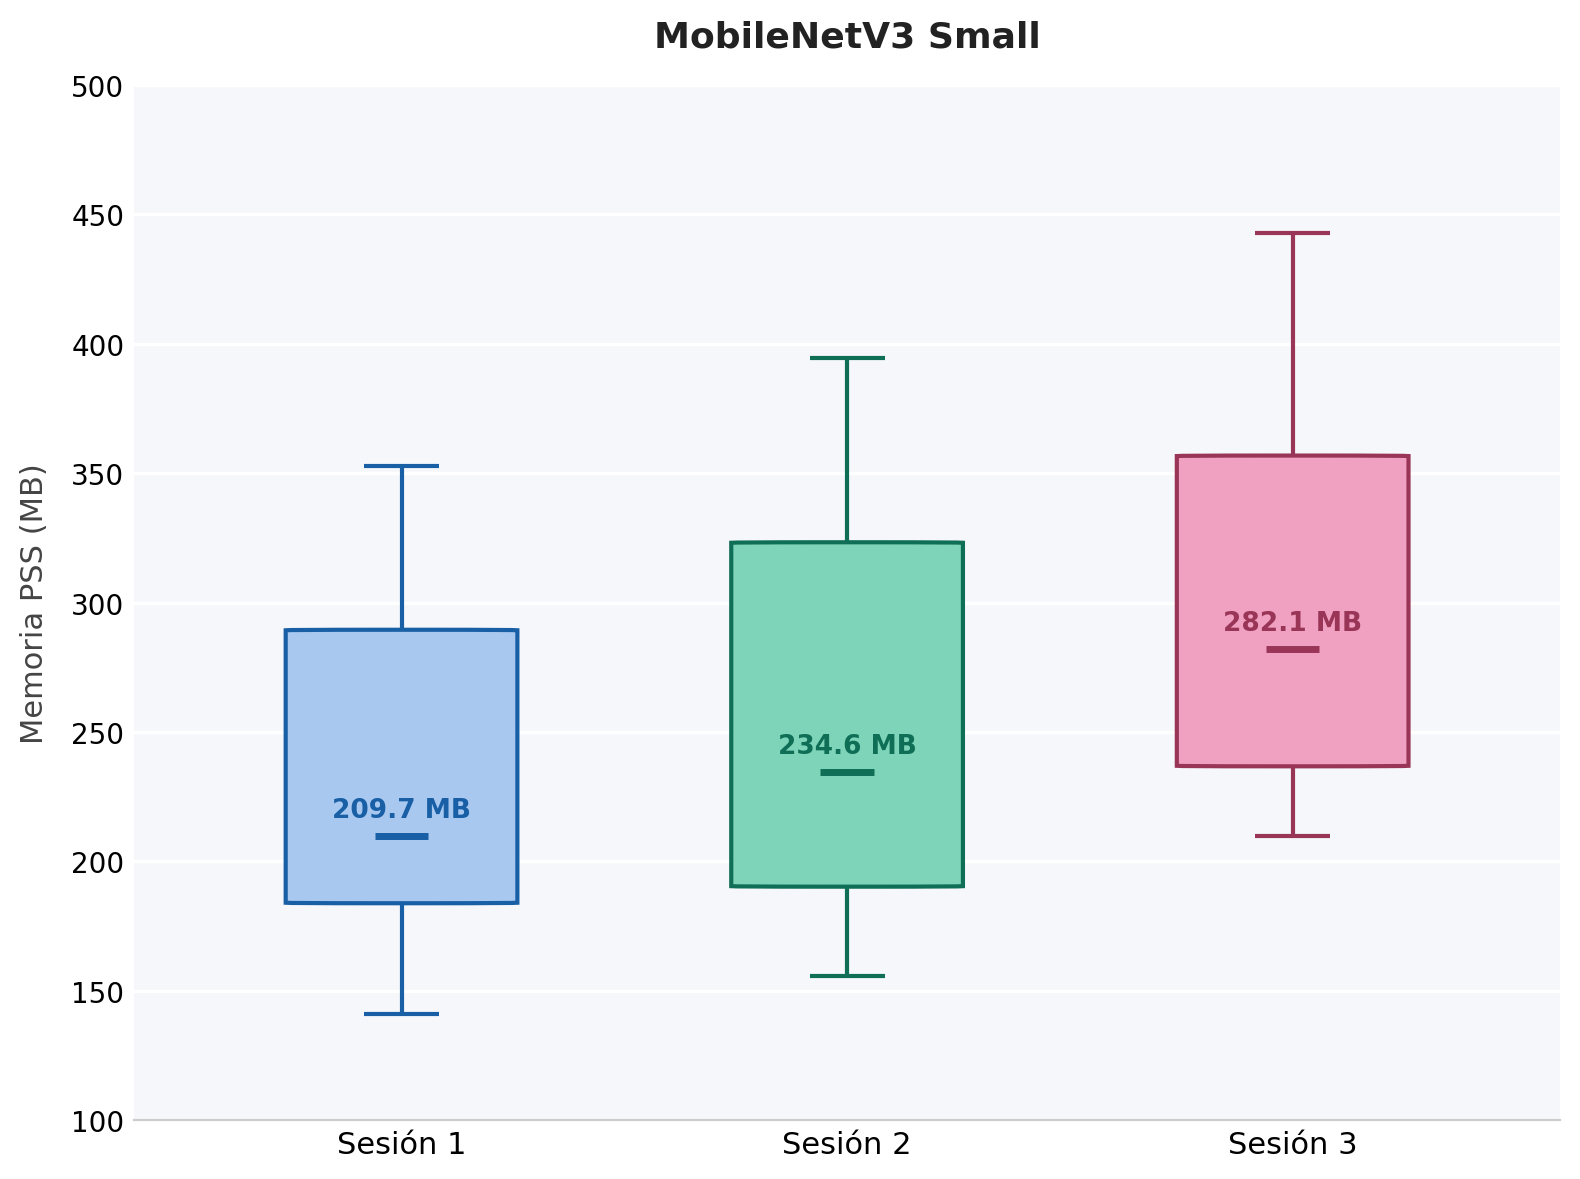
\includegraphics[width=\textwidth]{images/PSS_MobileNetV3Small_MotoG.png}
    \end{minipage}
    \hfill
    \begin{minipage}{0.49\textwidth}
        \centering
        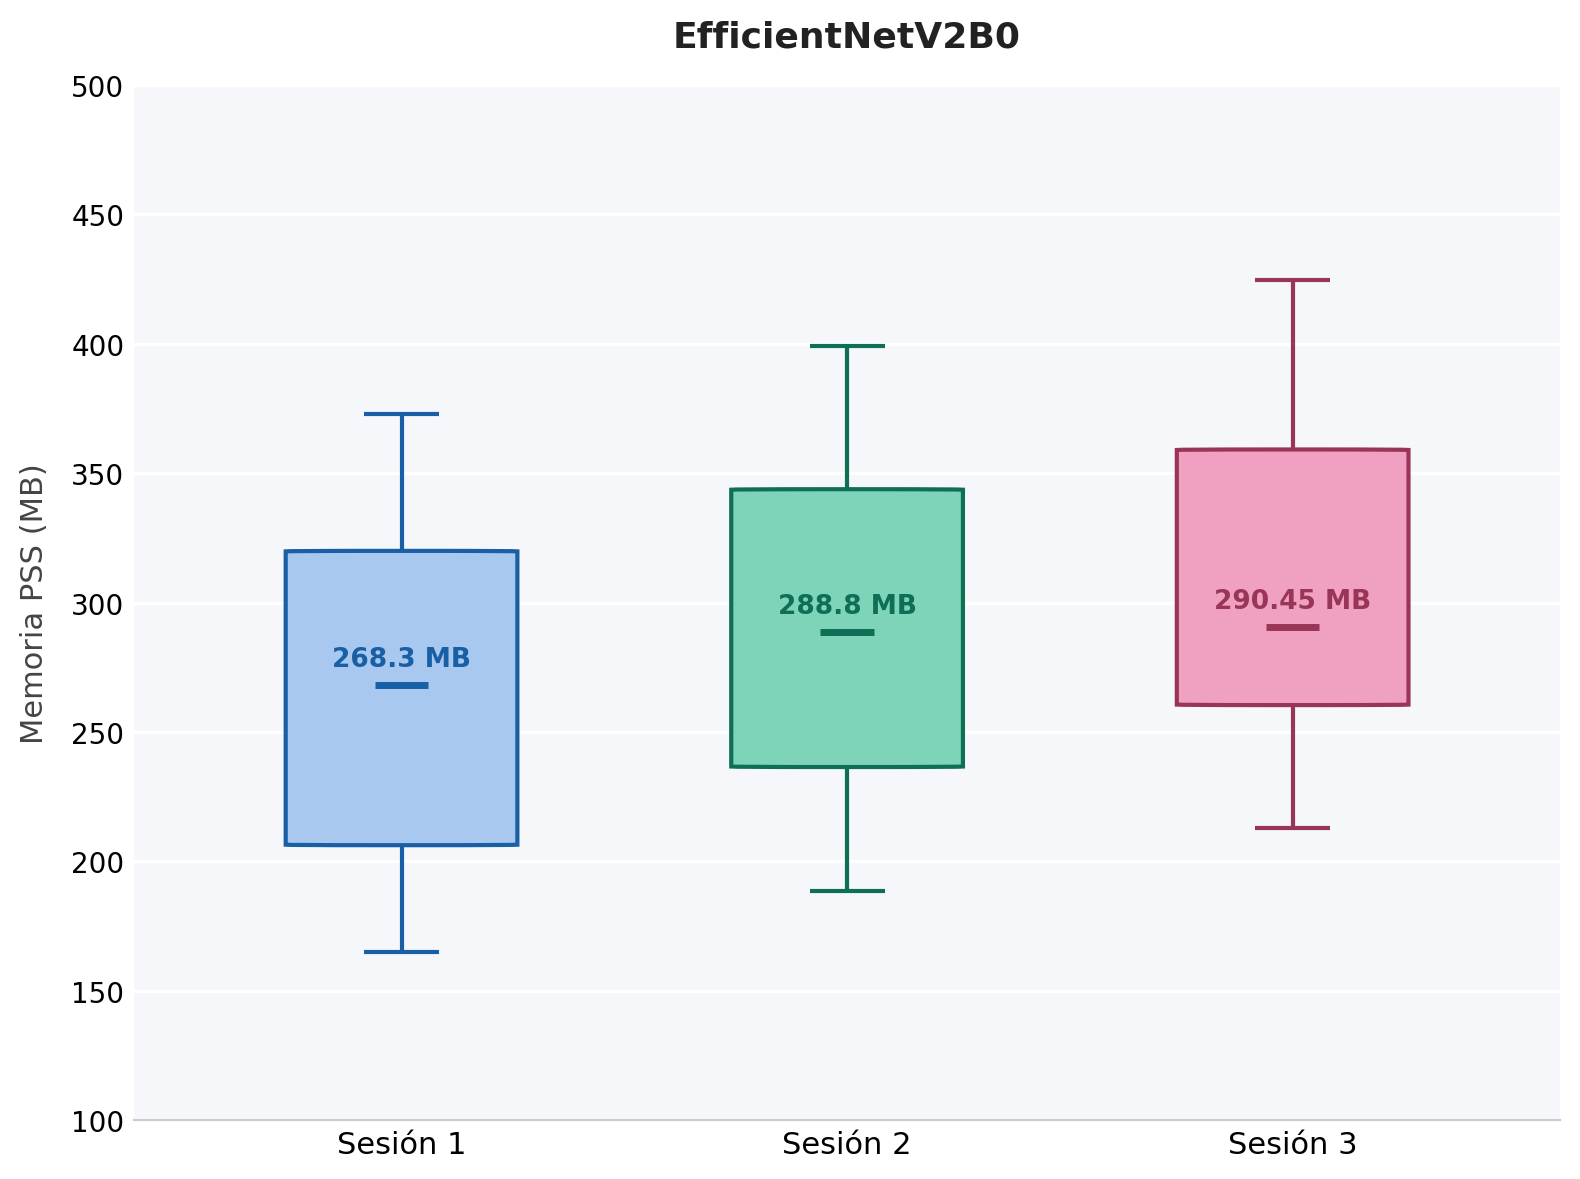
\includegraphics[width=\textwidth]{images/PSS_EfficientNetV2B0_MotoG.png}
    \end{minipage}
    \caption{Distribución de memoria PSS en Moto G30 para MobileNetV3 Small y EfficientNetV2B0.\label{fig:pss_motog_models}}
\end{figure}

La figura \ref{fig:pss_samsung_models} presenta la misma medición en el Samsung Galaxy S23, permitiendo comparar el comportamiento de
memoria de ambos modelos en un dispositivo con mayores recursos de hardware.

\begin{figure}[H]
    \centering
    \begin{minipage}{0.49\textwidth}
        \centering
        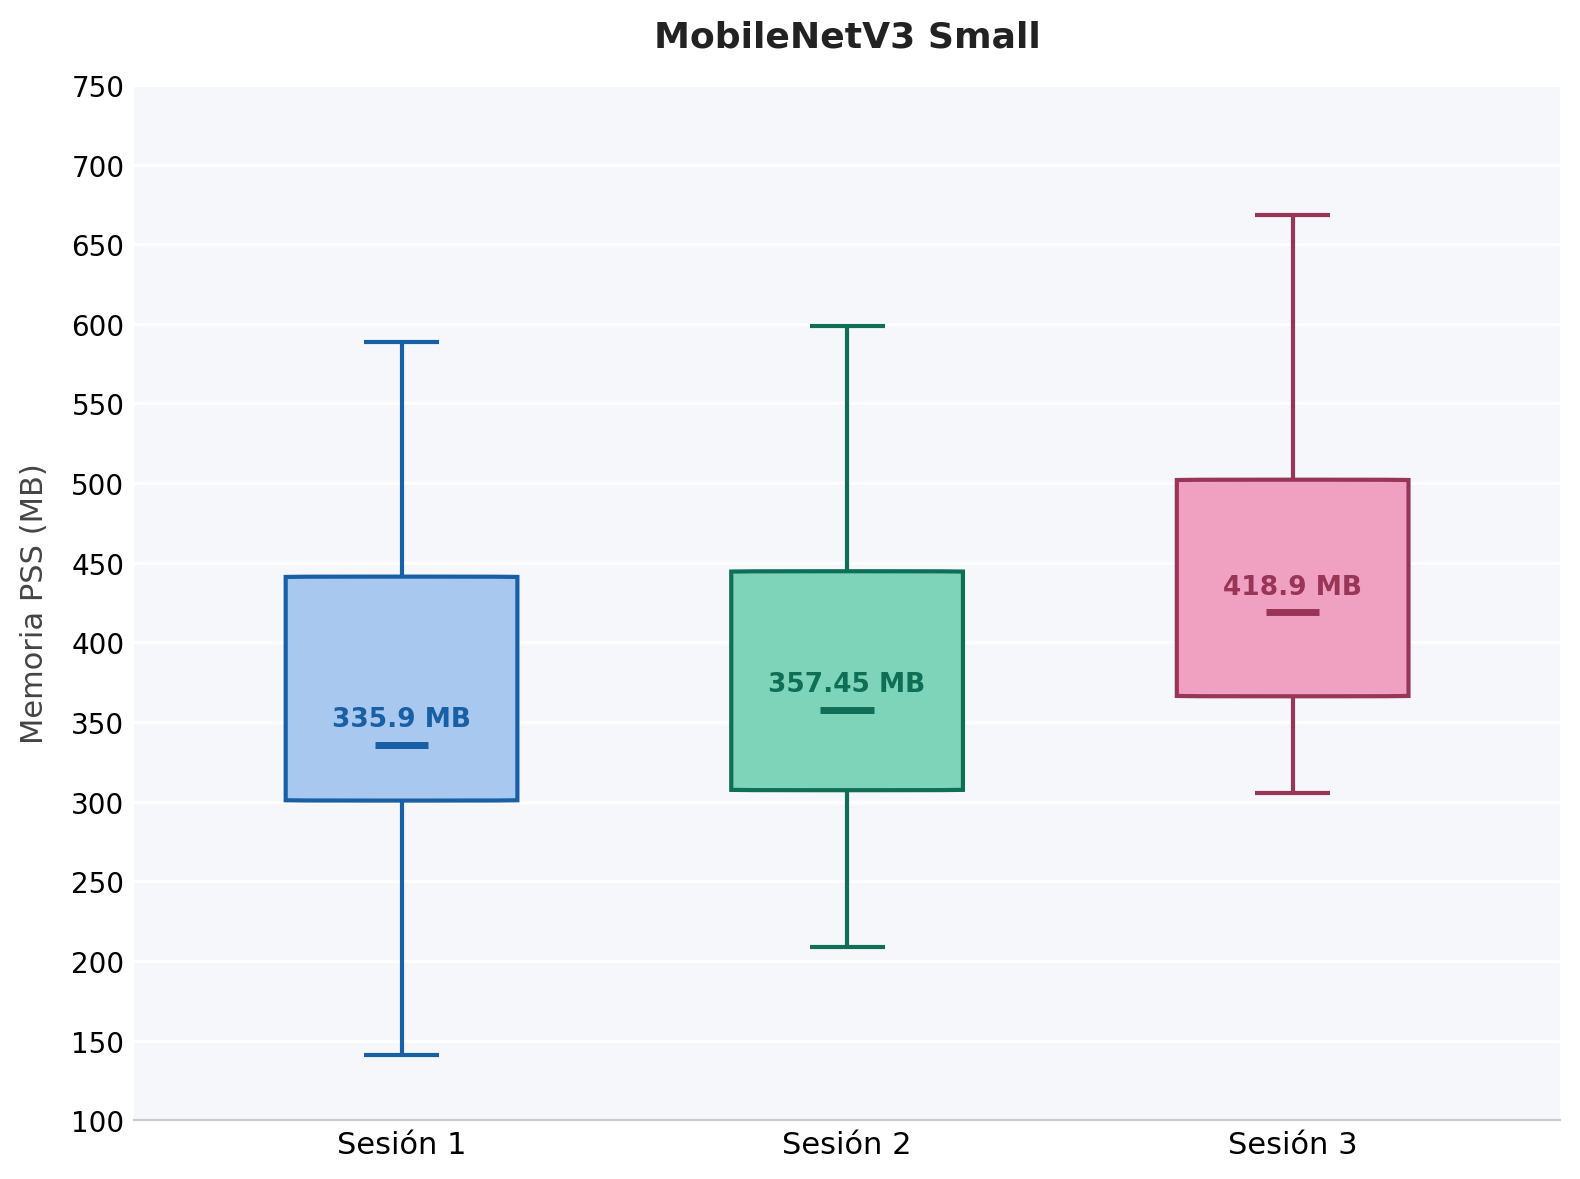
\includegraphics[width=\textwidth]{images/PSS_MobileNetV3Small_SamsungS23.png}
    \end{minipage}
    \hfill
    \begin{minipage}{0.49\textwidth}
        \centering
        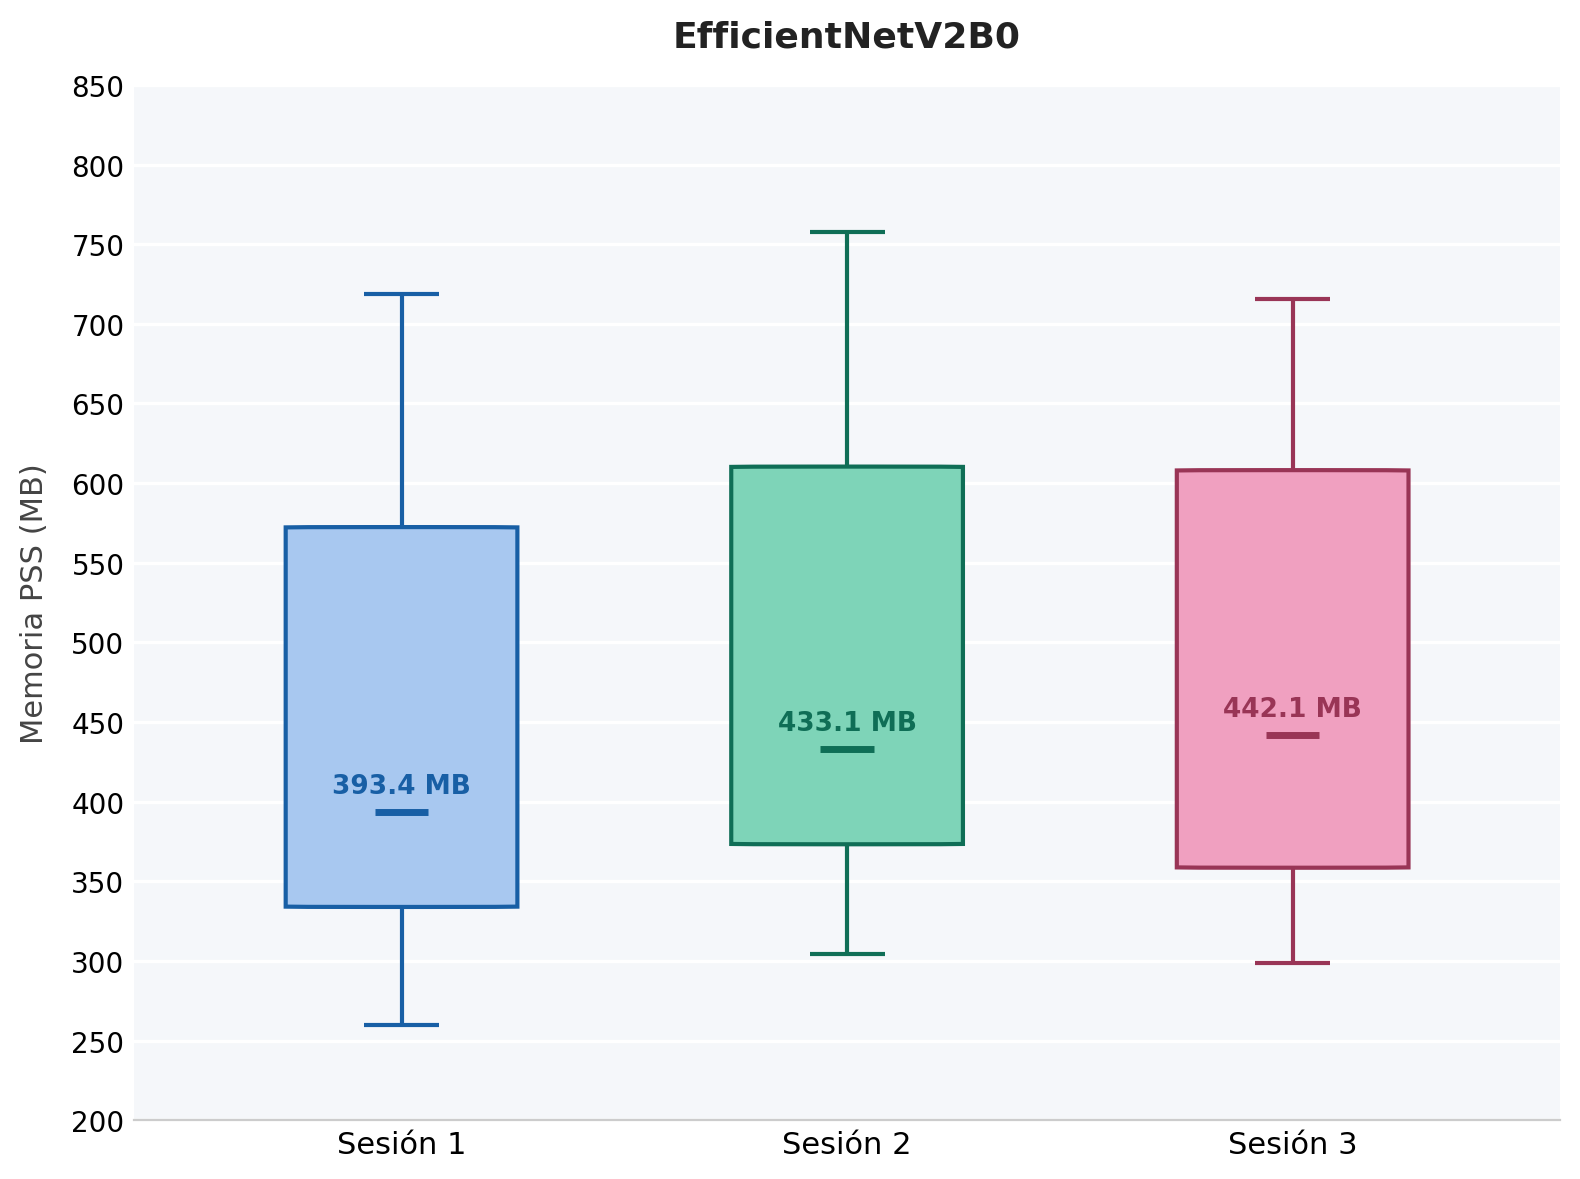
\includegraphics[width=\textwidth]{images/PSS_EfficientNetV2B0_SamsungS23.png}
    \end{minipage}
    \caption{Distribución de memoria PSS en Samsung Galaxy S23 para MobileNetV3 Small y EfficientNetV2B0.\label{fig:pss_samsung_models}}
\end{figure}


El consumo de memoria PSS en ambos dispositivos tiene una tendecia creciente durante la ejecucion de los modelos en las 3 sesiones de prueba, aunque con una variabilidad considerable. 
En el Moto G30, MobileNetV3 Small presentó un consumo promedio general de ~263 MB, mientras que EfficientNetV2B0 tuvo un consumo promedio de ~285 MB. En el Samsung
Galaxy S23, MobileNetV3 Small mostró un consumo promedio de ~394 MB, mientras que EfficientNetV2B0 registró un consumo promedio de ~466 MB. En ambos dispositivos, EfficientNetV2B0 presentó un 
consumo de memoria mayor que MobileNetV3 Small, lo cual es consistente con su arquitectura más compleja y su mayor número de parámetros.
El crecimiento progresivo de PSS a lo largo de la sesión indica acumulación de buffers intermedios. No se registraron OOM ni crashes en ninguna sesión.
Ademas se observa que el dispositivo Samsung al tener más RAM disponible (8 GB vs. 4 GB) el sistema operativo permite que la app ocupe más memoria sin presión.
Esto explica valores de PSS mayores en valor absoluto respecto al Moto G.


\subsection{Consumo de batería}

\subsection{Temperatura del dispositivo}

\subsection{Coherencia botánica}

En el dispositivo Moto G30, ambos modelos fueron consistentes es su clasificacion y confianza durante las tres sesiones de prueba, obteniendo el mismo 
diagnóstico para cada imagen evaluada. 
